\documentclass[10pt]{report}
\usepackage{kvmap}
\usepackage{listings} 
\usepackage{geometry}
\usepackage{tabularx}
\usepackage[framemethod=tikz]{mdframed}
 \geometry{
 a4paper,
 total={170mm,257mm},
 left=20mm,
 top=20mm,
 }
\usepackage{multicol}
\usepackage {graphicx}
\usepackage{karnaugh-map}
\begin{document}
\centering {
\includegraphics[scale=0.05]{logo.png}} \vspace{3mm}\\ \raggedright Name: T. Siva Gayathri\hspace{12cm}\\
\raggedleft Roll No.: FWC22037
\\ \centering \Large \textbf{ASSIGNMENT-1}\vspace{3mm}\normalsize\\ 
\begin{multicols}{2} 
\section{Question-2013 Section D Q6(d)}
Obtain the Minimal Form for the Boolean Expression:
H(P,Q,R,S)=$\sum(0,1,2,3,5,7,8,9,10,14,15)$
\section{Contents}
\raggedright
\textbf{Components}
\hspace{10em} 3
\\\textbf{Hardware}
\hspace{11.3em}   4
\\\textbf{Solution}
\hspace{12.1em}   5\\
\textit{Abstract-}
\textbf{This manual shows how to use 7447 BCD-seven segment display encoder to display Boolean Logic}
\section{Components}
\centering
\begin{tabular}{|l|c|c|}
\hline
Component & Value & Quantity\\
\hline
Resistor & 220 Ohm & 1\\
\hline
Arduino & UNO & 1\\
\hline
Seven Segment Display & & 1\\
\hline
Decoder & 7447 & 1\\
\hline
Jumper Wires & M-M & 20\\
\hline
Breadboard & & 1\\
\hline
\end{tabular}\\
\
\centerline{Table 3.0}
\section{Hardware}
\raggedright
1.Make connections between seven segment display and the 7447 ic as per the given table.\\
\
\centering
\\\begin{tabular}{|l|c|c|c|c|c|c|c|}
\hline
\textbf{7447} & a' & b' & c' & d' & e' & f' & g'\\
\hline
\textbf{Display} & a & b & c & d & e & f & g\\
\hline
\end{tabular}\\
\
\centerline{Table 4.0}\\
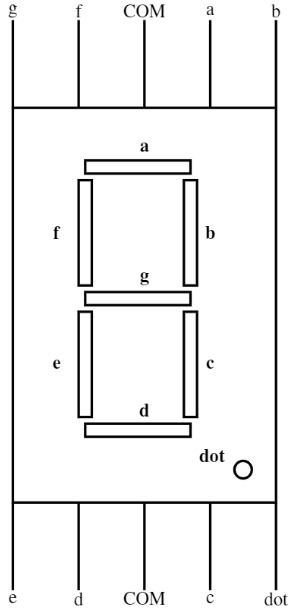
\includegraphics[scale=0.3]{sevenseg.jpeg}
\begin{center}
\centering\textbf{Figure 1: Pin diagram for Seven Segment}
\end{center}
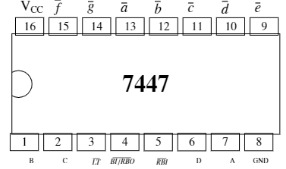
\includegraphics[scale=0.5]{ic.jpeg}
\begin{center}

\centering\textbf{Figure 2: Pin diagram for 7447} \\
\
\end{center}
\raggedright 
2.Make the connections between the Arduino and the 7447ic as per the given table.
\
\centering
\\\begin{tabular}{|l|c|c|c|c|}
\hline
\textbf{7447} & D & C & B & A\\
\hline
\textbf{Arduino} & 5 & 4 & 3 & 2\\
\hline
\end{tabular}\\
\
\centerline{Table 4.1}\\
\
\centering
\\\begin{tabular}{|l|c|c|c|c|}
\hline
& P & Q & R & S\\
\hline
\textbf{Input} & 0 & 1 & 1 & 0\\
\hline
\textbf{Arduino} & 6 & 7 & 8 & 9\\
\hline
\end{tabular}\\
\
\centerline{Table 4.2}
\raggedleft 3.In this we used the number 5 as an input to the Arduino and that would give the output as 1. 
\newpage
\centering
\section{Solution} 
\centering
\textbf{Truth Table}\\
\
\\\begin{tabular}{|c|c|c|c|c|}
\hline
\textbf{P} & \textbf{Q} & \textbf{R} & \textbf{S} & \textbf{H}\\
\hline
0 & 0 & 0 & 0 & 1\\
\hline
0 & 0 & 0 & 1 & 1\\
\hline
0 & 0 & 1 & 0 & 1\\
\hline
0 & 0 & 1 & 1 & 1\\
\hline
0 & 1 & 0 & 0 & 0\\
\hline
0 & 1 & 0 & 1 & 1\\
\hline
0 & 1 & 1 & 0 & 0\\
\hline
0 & 1 & 1 & 1 & 1\\
\hline
1 & 0 & 0 & 0 & 1\\
\hline
1 & 0 & 0 & 1 & 1\\
\hline
1 & 0 & 1 & 0 & 1\\
\hline
1 & 0 & 1 & 1 & 0\\
\hline
1 & 1 & 0 & 0 & 0\\
\hline
1 & 1 & 0 & 1 & 0\\
\hline
1 & 1 & 1 & 0 & 1\\
\hline
1 & 1 & 1 & 1 & 1\\
\hline
\end{tabular}\\
\
\centerline{Table 5.0}
\raggedright 1.The following K-map is obtained from the above truth table.\\
\raggedright 2.As we have Four Variables we obtain a 16 cell K-Map\\
\centering
\begin{kvmap}
    \begin{kvmatrix}{R,S,P,Q}
    1 & 1 & 1 & 1\\
    0 & 1 & 1 & 0\\
    0 & 0 & 1 & 1\\
    1 & 1 & 0 & 1\\
    \end{kvmatrix}
\end{kvmap}\\
\centerline{Table 5.1}
\raggedright 3.Now we do grouping to obtain the minimal expression using the K-Map.\\
\centering
\begin{kvmap}
    \begin{kvmatrix}{R,S,P,Q}
    1 & 1 & 1 & 1\\
    0 & 1 & 1 & 0\\
    0 & 0 & 1 & 1\\
    1 & 1 & 0 & 1\\
    \end{kvmatrix}
    \bundle[color=red,invert=true]{0}{0}{3}{0}
    \bundle[color=red,invert=true]{0}{3}{3}{3}
    \bundle[color=blue]{1}{0}{2}{1}
\end{kvmap}\\
\
\centerline{Table 5.2}
\raggedright The minterm expression for the two groupings are $\overline{QS}$ and $\overline{P}$S\\
\centering
\begin{kvmap}
    \begin{kvmatrix}{R,S,P,Q}
    1 & 1 & 1 & 1\\
    0 & 1 & 1 & 0\\
    0 & 0 & 1 & 1\\
    1 & 1 & 0 & 1\\
    \end{kvmatrix}
    \bundle[color=violet]{2}{2}{3}{2}
    \bundle[color=cyan]{0}{3}{1}{3}
\end{kvmap}
\centerline{Table 5.3}
\raggedright The minterm expression for the two groupings are PQR and P$\overline{QR}$\\
\centering
\begin{kvmap}
    \begin{kvmatrix}{R,S,P,Q}
    1 & 1 & 1 & 1\\
    0 & 1 & 1 & 0\\
    0 & 0 & 1 & 1\\
    1 & 1 & 0 & 1\\
    \end{kvmatrix}
    \bundle[color=red,invert=true]{0}{0}{3}{0}
    \bundle[color=red,invert=true]{0}{3}{3}{3}
    \bundle[color=blue]{1}{0}{2}{1}
    \bundle[color=violet]{2}{2}{3}{2}
    \bundle[color=cyan]{0}{3}{1}{3}
\end{kvmap}\\
\centerline{Table 5.4}
\raggedright The Minimal expression is \\ H = $\overline{QS}$+$\overline{P}$S+PQR+P$\overline{QR}$S\\
\raggedright 4.Download the code from the given link and upload to the Arduino.\\
\begin{mdframed}
 https://github.com/siva-gayathri/FWC/blob/main
 \\/assignment-1/codes/src/main.cpp
\end{mdframed}
\raggedright 5.Go to the working directory
execute pio run and pio run -t upload.\\
6.Whenever you change the inputs you will see the respective output. 
\end{multicols}
\end{document}